\clearpage

\section{Implementation}

This section provides a comprehensive overview of the system's implementation. It includes the user interface illustrating each component and feature implemented in our email marketing tool during the third sprint. The user interface was designed to be simple and user-friendly. The goal was to make the tool easy to use even for users without much technical expertise.

\subsection{Upload Media}
The \textit{Upload Media} feature allows users to either drop a media file or select one to upload from their device. Once uploaded, these media files will be available in the email builder to create email templates with images. This feature ensures that users can easily access and use their media assets when designing their email campaigns.

\begin{figure}[ht]
\centering
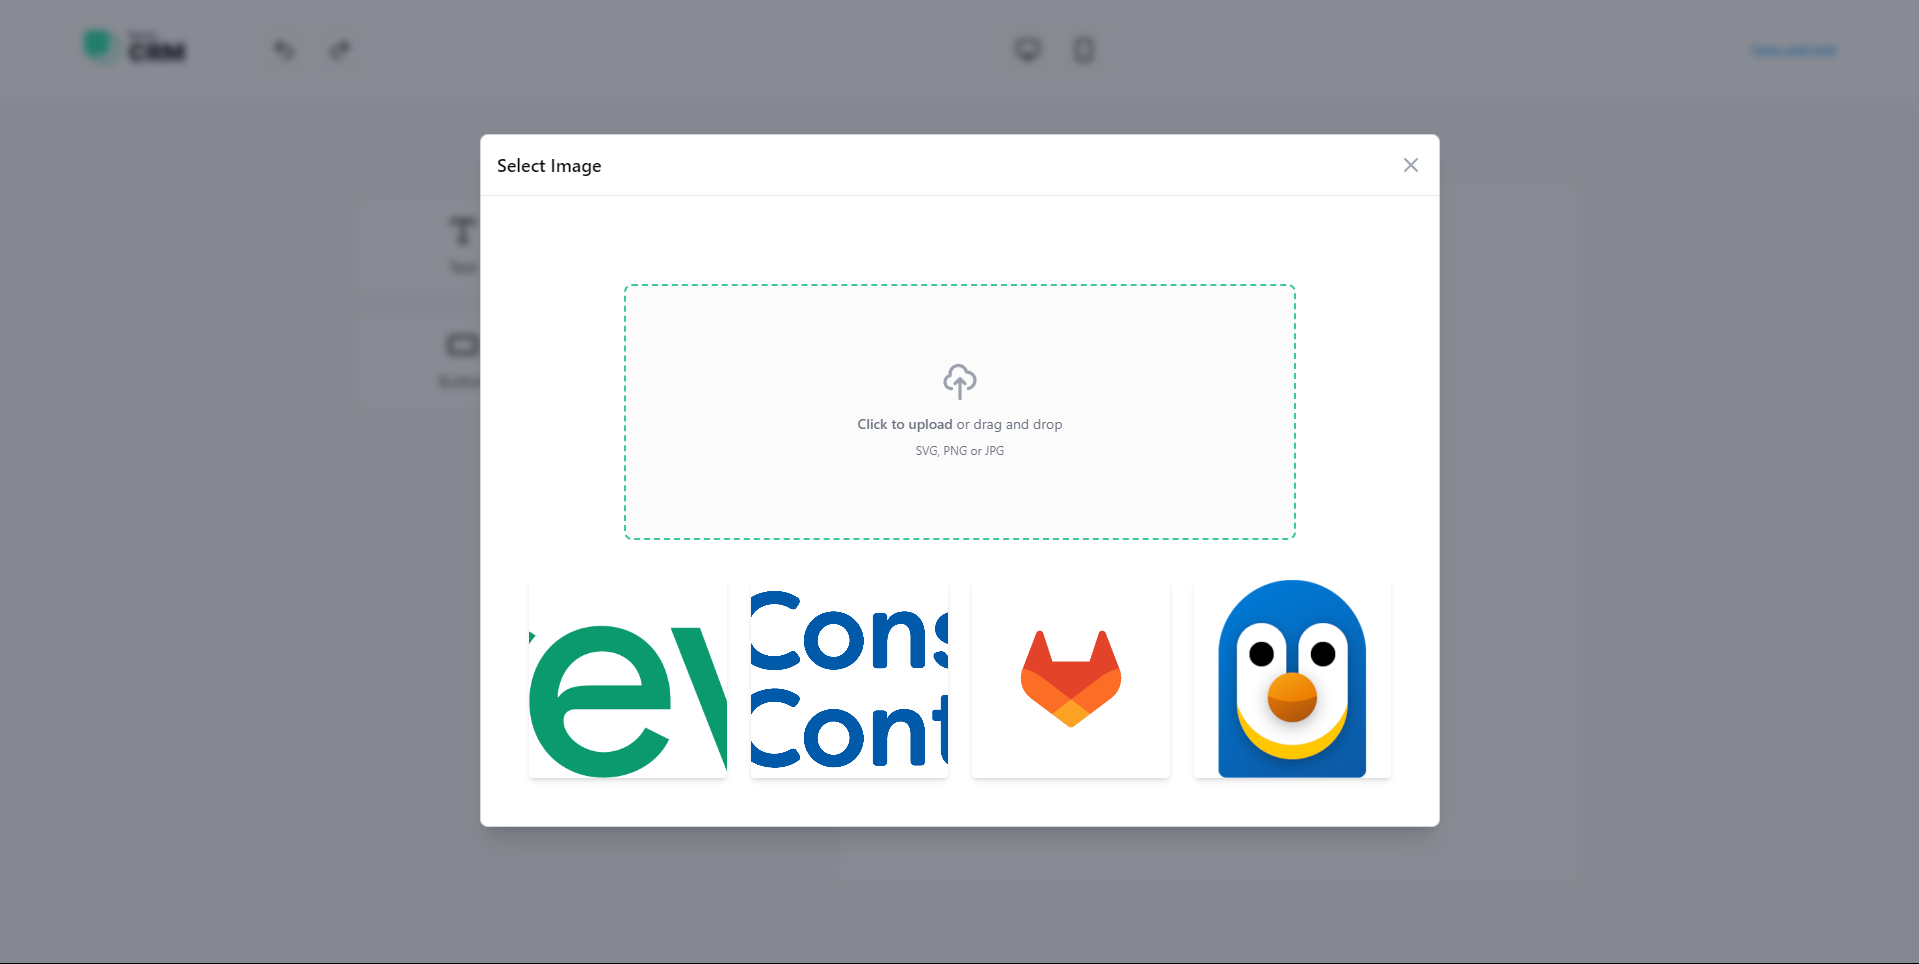
\includegraphics[width=0.8\textwidth]{Images/sprint2/screenshots/Screenshot 2024-06-06 004807.png}
\caption{User Interface for Upload Media}
\end{figure}

\subsection{Create New Organization}
The \textit{Create New Organization} feature functions as a workspace where every organization has its own campaigns, templates library, media cloud, and audience. By default, the creator of the organization becomes the admin. This setup ensures that each organization operates independently and securely with dedicated resources.

\begin{figure}[ht]
	\centering
	\begin{subfigure}[b]{0.45\linewidth}
		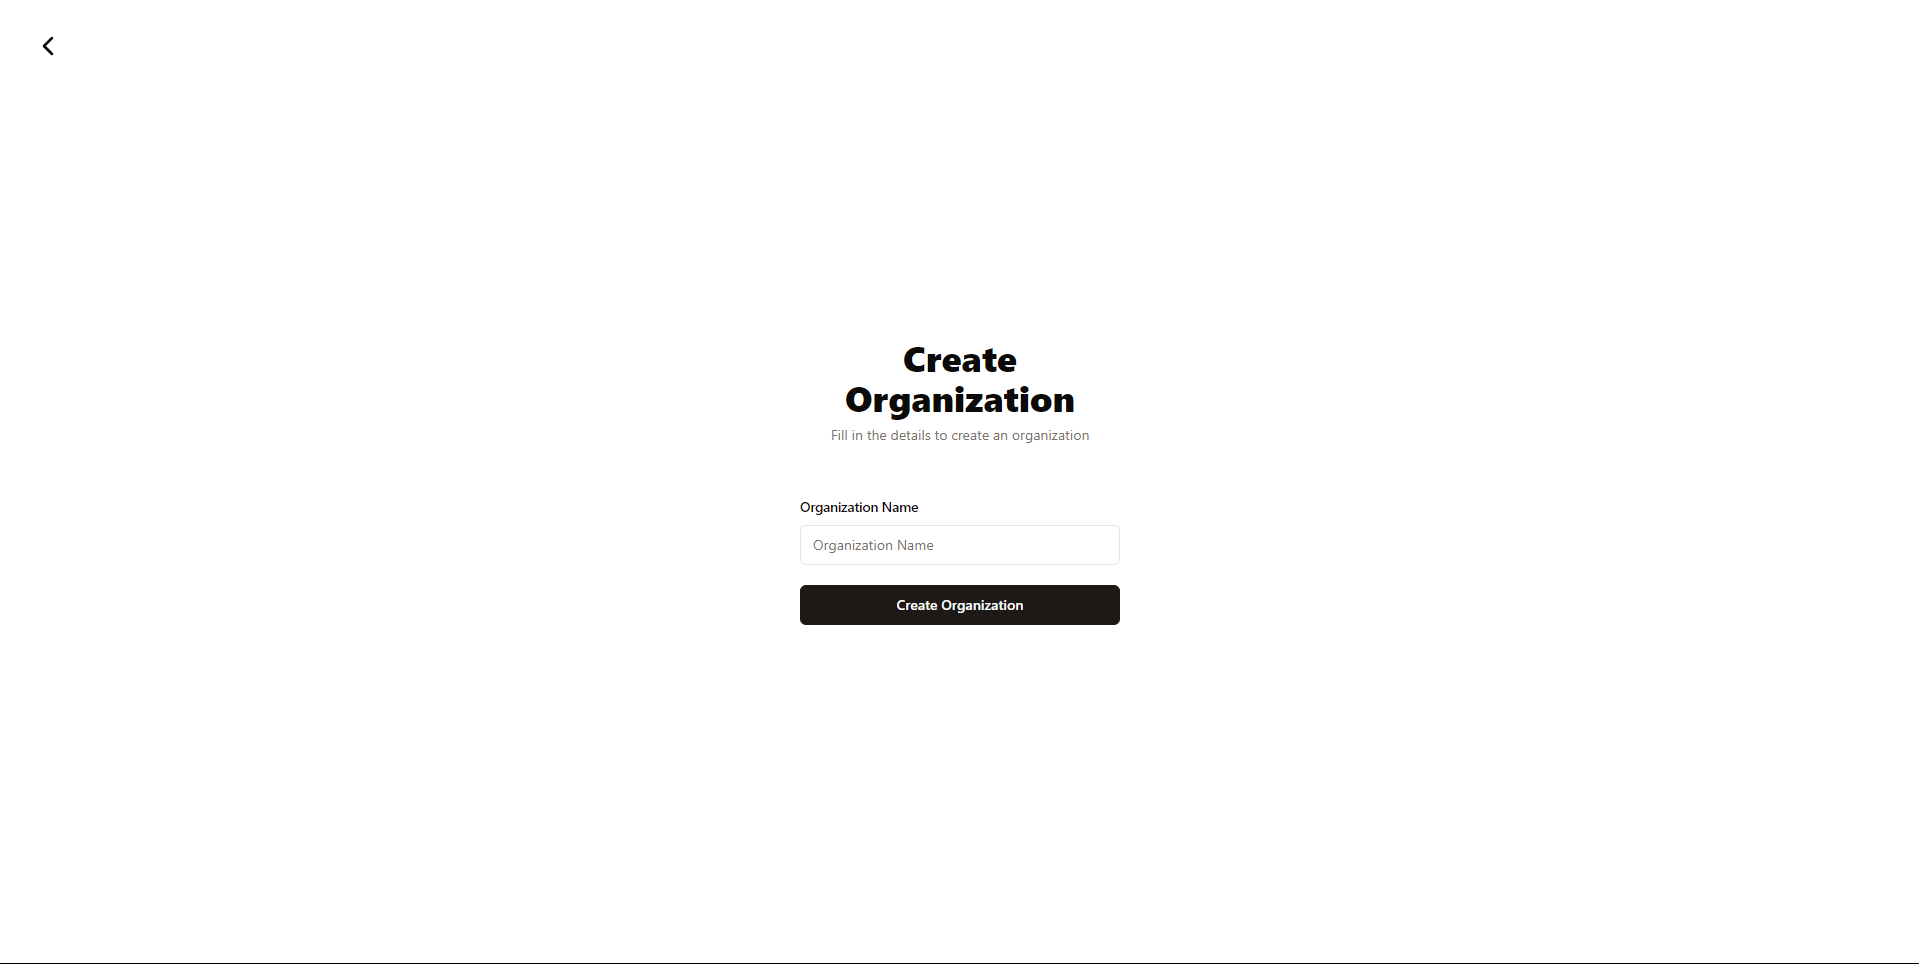
\includegraphics[width=\linewidth]{Images/sprint2/screenshots/Screenshot 2024-06-06 004648.png}
		\caption{Create New Organization}
		\label{fig:Create New Organization}
	\end{subfigure}
	\hfill
	\begin{subfigure}[b]{0.45\linewidth}
		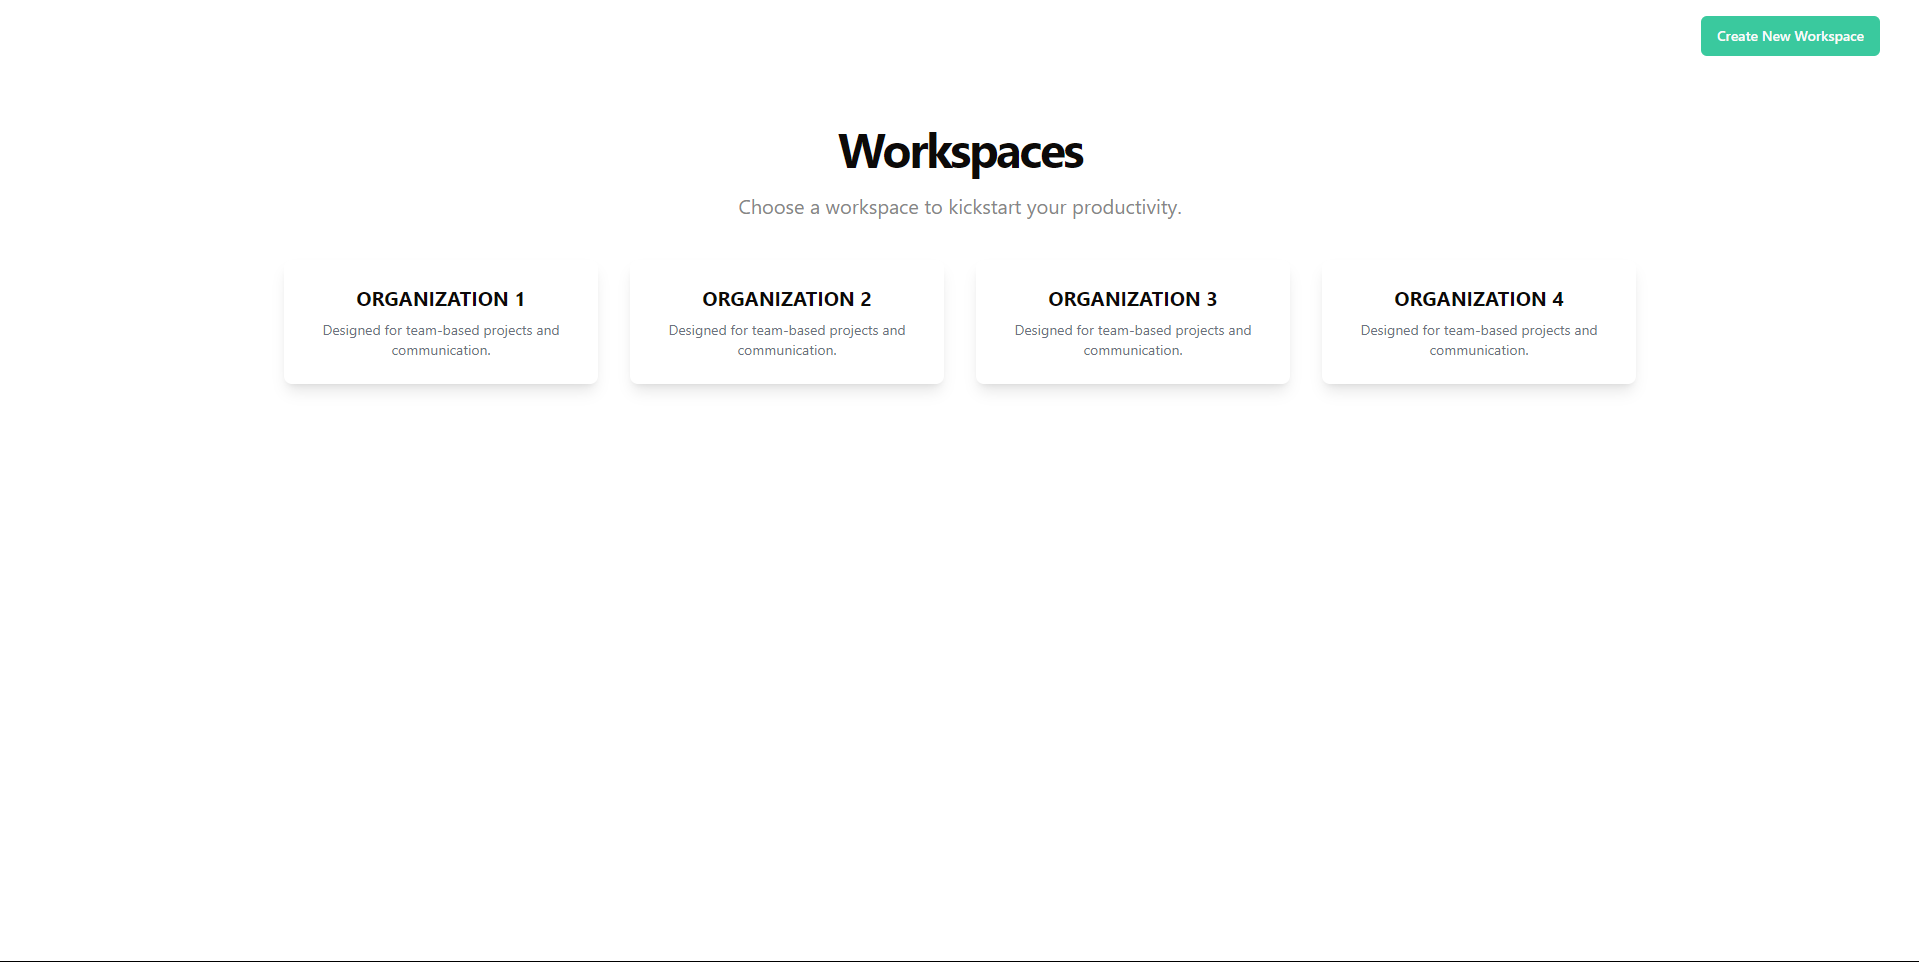
\includegraphics[width=\linewidth]{Images/Sprint2/screenshots/Screenshot 2024-06-06 004720.png}
		\caption{Selcting Organization's Workspace}
		\label{fig:Selcting Organization's Workspace}
	\end{subfigure}
	\caption{User Interface for Creating a New Organization}
\end{figure}

\subsection{Invite New Members to Join Organization}
The \textit{Invite New Members} feature allows the admin of an organization to send an email invitation link with a unique token to targeted users to join the organization. Upon sending an invitation, the targeted user is saved in the database with a "PENDING" status. If the user clicks on the sent link, their status changes to "ACCEPTED". If the invitation is not accepted within a day, it will be declined.

\begin{figure}[ht]
\centering
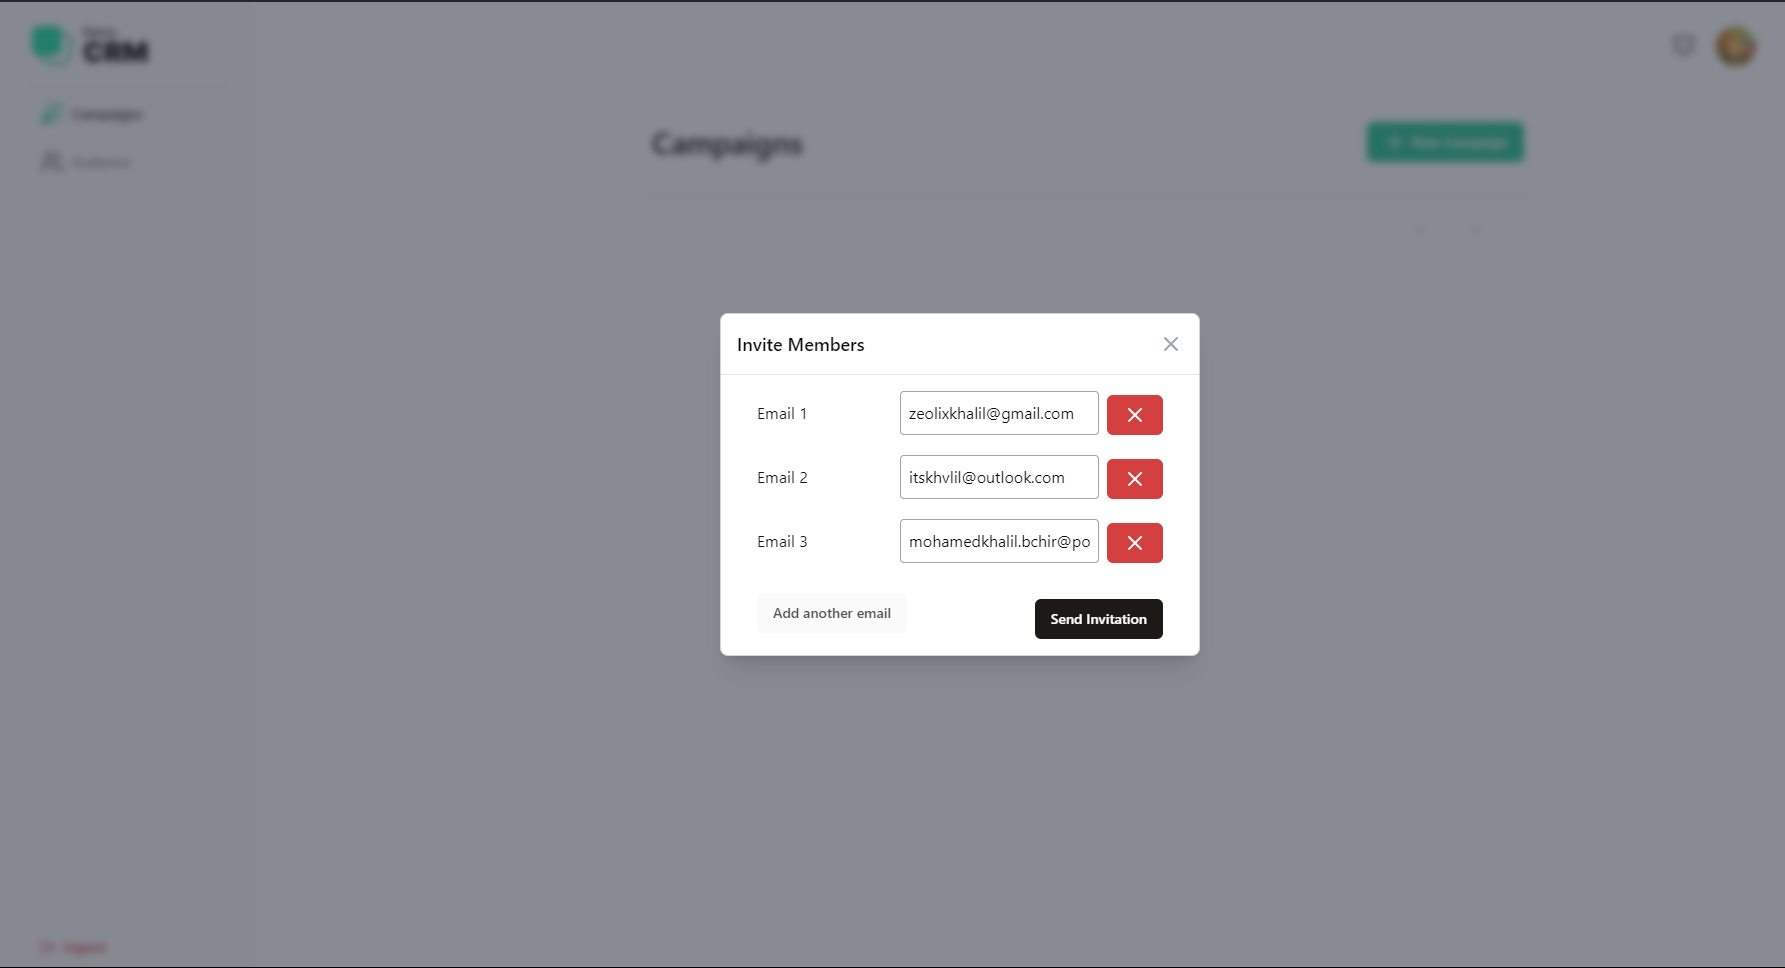
\includegraphics[width=0.8\textwidth]{Images/sprint2/screenshots/Screenshot 2024-06-06 004557.png}
\caption{User Interface for Inviting New Members}
\end{figure}

\subsection{Manage Members And Roles Within an Organization}
\paragraph*{Assign Roles}
The \textit{Assign Roles} feature allows the admin to update the role of any member within the organization. Each role comes with specific permissions, enabling the admin to control the level of access and actions that different members can perform within the organization.

\paragraph*{Remove Members}
The \textit{Remove Members} feature enables the admin to remove a user from the organization by clicking on the remove icon. When a user is removed, their status is updated to "INACTIVE", ensuring that their data is not lost and can be reactivated if needed in the future.

\begin{figure}[ht]
\centering
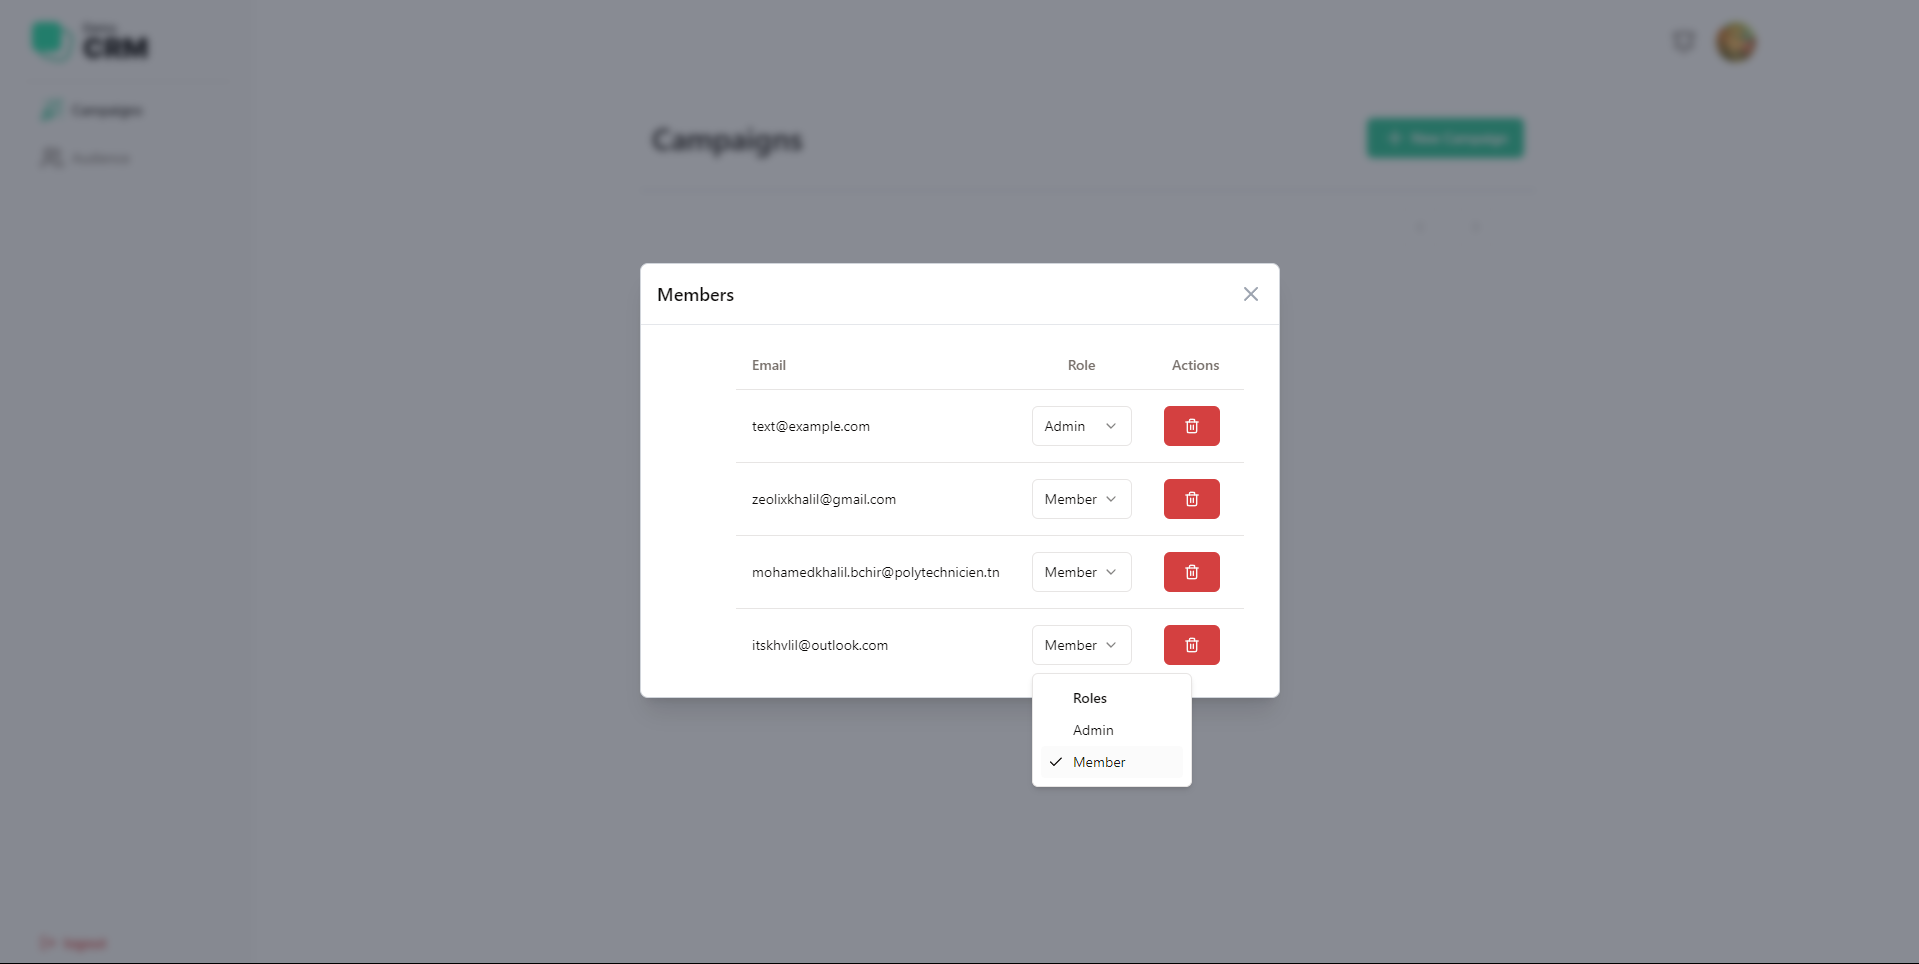
\includegraphics[width=0.8\textwidth]{Images/sprint2/screenshots/Screenshot 2024-06-06 004631.png}
\caption{User Interface for Assigning Roles And Managing Members}
\label{fig:User Interface for Assigning Roles And Managing Members}
\end{figure}

